\documentclass[hidelinks, a4paper, 11pt]{scrartcl}

% Use-Packages:
\usepackage[utf8]{inputenc}
\usepackage{graphicx}
\usepackage{color}
\usepackage{hyperref}
\usepackage{enumerate}

% Defined short commands please here
\def\app{''Decision Maker''}

% Headings
\pagestyle{myheadings}
\markright{Project: \app}

\makeatletter

\author{Rashad Asgarbayli,\\ Kanan Ibrahimov,\\ Philipp Schoch}

\title{\vspace{3cm}
\includegraphics[scale=0.7]{Logo.png}\\ \app\vspace{20mm}}

\subtitle{Functional Specifications Document}

\date{\today}

\begin{document}

\maketitle
\thispagestyle{empty}

\newpage

\pagenumbering{roman}
\tableofcontents

\newpage

\pagenumbering{arabic}

\section{Introduction}

\paragraph{}Can't decide what to eat? Can't decide where to go with friends? Can't decide what to wear? Can't decide which pupil answers the lesson? Sometimes because of the multiple available options, we need help to decide something. An Application that makes random decisions could help You to do that and ease down. We introducing our new application called \app. The app can generate a number for the inputted interval (for example: number of the item in menu or number of the pupil in the list) or make a decision for the inputted list (for example: decide among ''go to the restaurant'', ''go to the park'', ''go to the cinema'' etc.). Need democratic selection without revealing the names? Multiple users can input their proposals over bluetooth or network and after \app makes a decision, everyone becomes the same result without knowing who wrote the proposal. What You need to do? Simply enter what You want to decide and shake the handy. That's all. Now You have Your answer. It is so simple.

\newpage
\section{Objectives}

\paragraph{}Blablabla

\subsection{Mandatory Criteria}

\begin{itemize}
\item Blablabla
\item Blablabla
\item Blablabla
\end{itemize}

\subsection{Facultative Criteria}

\begin{itemize}
\item Blablabla
\item Blablabla
\item Blablabla
\end{itemize}

\subsection{Excluded Criteria}

\begin{itemize}
\item Blablabla
\item Blablabla
\item Blablabla
\end{itemize}


\newpage
\section{Product Usage}
   This section of the requirements is about the user groups of the system. It will be described how, why and by whom the \app will be used. 

\subsection{Blablabla}
\paragraph{}Blablabla

\subsection{Blablabla}
\paragraph{}Blablabla


\newpage
\section{Product Environment}
\subsection{Environment for Blablabla}
\paragraph{}Blablabla

\subsection{Hardware}
\paragraph{}Minimum System Requirements	 
\begin{itemize}
\item Blablabla
\item Blablabla
\item Blablabla
\end{itemize}
	 
\subsection{Mobile Environment Criteria}
\paragraph{}The minimum Android version needed to run the \app is Android Blablabla


\newpage
\section{Functional Requirements}

\begin{description}
\item[/F010/ Choice from Interval]\hfill \\ User inputs minimum and maximum numbers, then program generates a number between these.
\item[/F020/ Choice from Strings]\hfill \\ User or users input at least two Strings for random choice, then program chooses one of them.
\item[/F030/ BlaBlaBla]\hfill \\ Blablabla
\end{description}

\newpage
\section{Nonfunctional Requirements}

\begin{description}
\item[/NF010/ BlaBlaBla]\hfill \\ Blablabla
\item[/NF020/ BlaBlaBla]\hfill \\ Blablabla
\item[/NF030/ BlaBlaBla]\hfill \\ Blablabla
\end{description}

\newpage
\section{Product Data}

\subsection{Essential data}
\begin{description}
\item[/D010/ BlaBlaBla]\hfill \\ Blablabla
\item[/D020/ BlaBlaBla]\hfill \\ Blablabla
\item[/D030/ BlaBlaBla]\hfill \\ Blablabla
\end{description}

\subsection{Facultative data}
\begin{description}
\item[/D010/ BlaBlaBla]\hfill \\ Blablabla
\item[/D020/ BlaBlaBla]\hfill \\ Blablabla
\item[/D030/ BlaBlaBla]\hfill \\ Blablabla
\end{description}


\newpage
\section{Global Test Cases and Scenarios}

In this section we describe the tests for the functional requirements in steps and with the wanted outcome. 

\subsection{Basic features}
\begin{description}
\item[/TB010/ BlaBlaBla]\hfill \\ Blablabla
\item[/TB020/ BlaBlaBla]\hfill \\ Blablabla
\item[/TB030/ BlaBlaBla]\hfill \\ Blablabla
\end{description}

\subsection{Optional features}
\begin{description}
\item[/TO010/ BlaBlaBla]\hfill \\ Blablabla
\item[/TO020/ BlaBlaBla]\hfill \\ Blablabla
\item[/TO030/ BlaBlaBla]\hfill \\ Blablabla
\end{description}

\newpage
\section{System Model}

\begin{figure}[h!]
\centering
%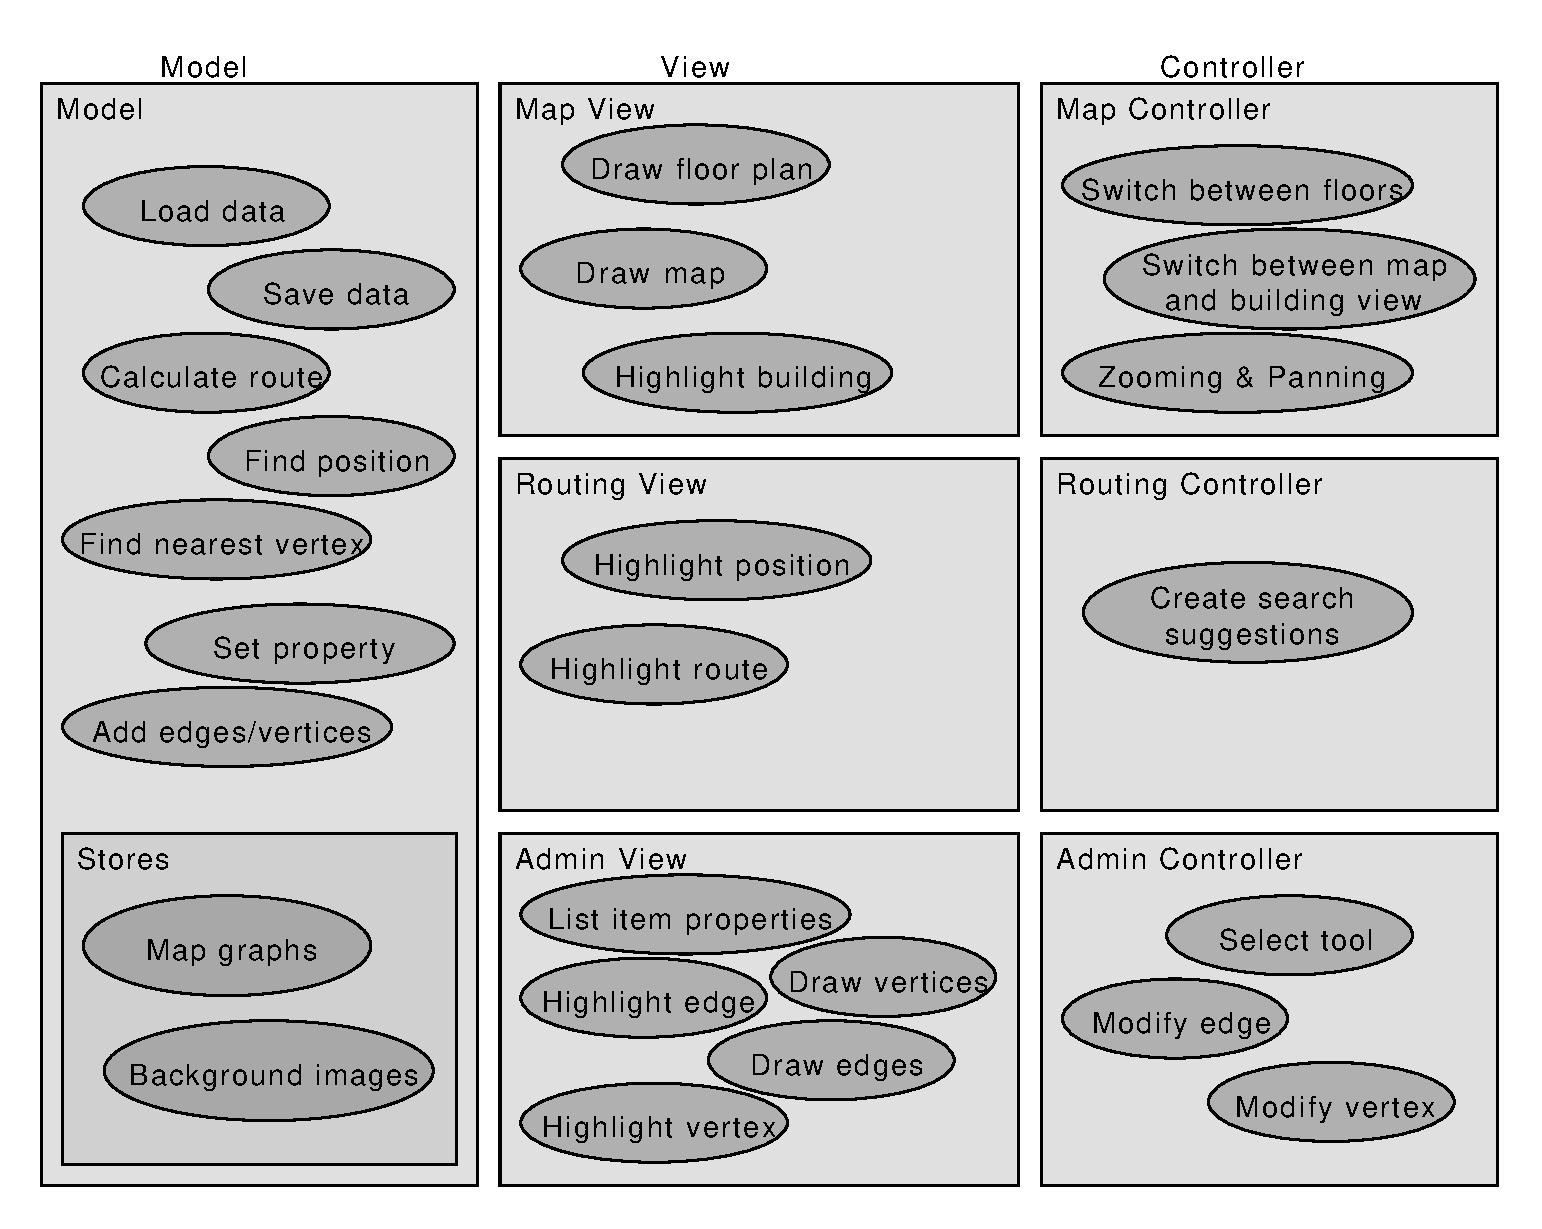
\includegraphics[width=0.8\textwidth]{mvc.png}
\caption{System Model}
\end{figure}

\paragraph{}The main model applied to the product is the
model-view-controller (MVC model).

\paragraph{}Blablabla

\subsection{Graphical User Interface}

\paragraph{}Blablabla

\begin{figure}[h!]
\centering
%\includegraphics[width=0.8\textwidth]{gui.png}
\caption{GUI Blablabla}
\end{figure}


\newpage
\section{Glossary}

\begin{description}
\item[GUI]\hfill \\ Graphical User Interface
\item[BlaBlaBla]\hfill \\ Blablabla
\item[BlaBlaBla]\hfill \\ Blablabla
\item[BlaBlaBla]\hfill \\ Blablabla
\end{description}

\end{document}
